%label:"fig:liuvilleMomentMapR2"
%author:JeffHicks
%name:"Liouville structure on $\CC^2$ as viewed from the moment map"
%type:"figure"
%parent:"exm:contactManifold"
%caption:"The Liouville structure on $\CC^2$ as viewed from the moment map"


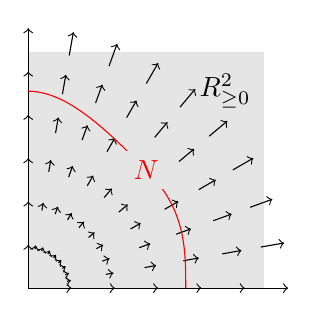
\begin{tikzpicture}
    \fill[gray!20] (0,0)--(3, 0)--(3,3)--(0,3)--cycle;
    \draw (0,0)--(3,0) (0,3)--(0,0);
    \foreach \r in { .5, 1,1.5, 2,2.5, 3} {
        \foreach \t in {0,...,9} {
            \draw[->] ({\r * cos(10*\t)},{ \r * sin(10*\t) })-- ({1.1*\r * cos(10*\t)},{ 1.1*\r * sin(10*\t) });
            }
    }
    
    \draw[red] (0,2.5) .. controls (0.5,2.5) and (1,2) .. (1.5,1.5) node[fill=gray!20] {$N$} .. controls (2,1) and (2,0.5) .. (2,0);
    \node at (2.5, 2.5) {$\mathbb R_{\geq 0}^2$};
    \end{tikzpicture}